\chapter{Homogeneous Catalysis in Industry}\label{ch:b3:homogeneous-catalysis}

Most of the world's acetic acid, the raw material of vinyl acetate, of
cellulose acetate and of the purified terephthalic acid of plastic bottles, is
made from methanol and carbon monoxide in a few very large plants. In each, a
rhodium or iridium complex dissolved at low concentration in the reaction
liquid turns over thousands of times an hour, for years. The same kind of
chemistry hydrogenates, adds CO and hydrogen to alkenes, exchanges the ends of
double bonds, joins aromatic rings and makes polyethylene and polypropylene by
the million tonnes. This chapter reads the catalytic cycles of the main
industrial processes with the tools of \cref{ch:b3:organometallic-bonding}:
electron counts, oxidation states, rate-determining steps, and the symmetry of
the catalyst that sets the structure of a polymer.

\begin{recall}
The Year 2 volume introduced the elementary steps of organometallic reactions
(oxidative addition, reductive elimination, migratory insertion, $\beta$-hydride
elimination, transmetalation), catalytic cycles, precatalysts, turnover number
and frequency, and read the cycles of hydrogenation, \omterm{def:b3:homogeneous-catalysis:hydroformylation}{hydroformylation} and
cross-coupling; it also defined tacticity and chain-growth polymerisation,
conversion and selectivity. \Cref{ch:b3:organometallic-bonding} counted
electrons and described carbonyl and \omterm{def:b3:organometallic-bonding:carbene}{carbene} ligands;
\cref{ch:b3:complex-kinetics} gave saturation kinetics;
\cref{ch:b3:point-groups} the \omterm{def:b3:point-groups:operation}{symmetry elements} of molecules.
\end{recall}

\begin{omfigure}
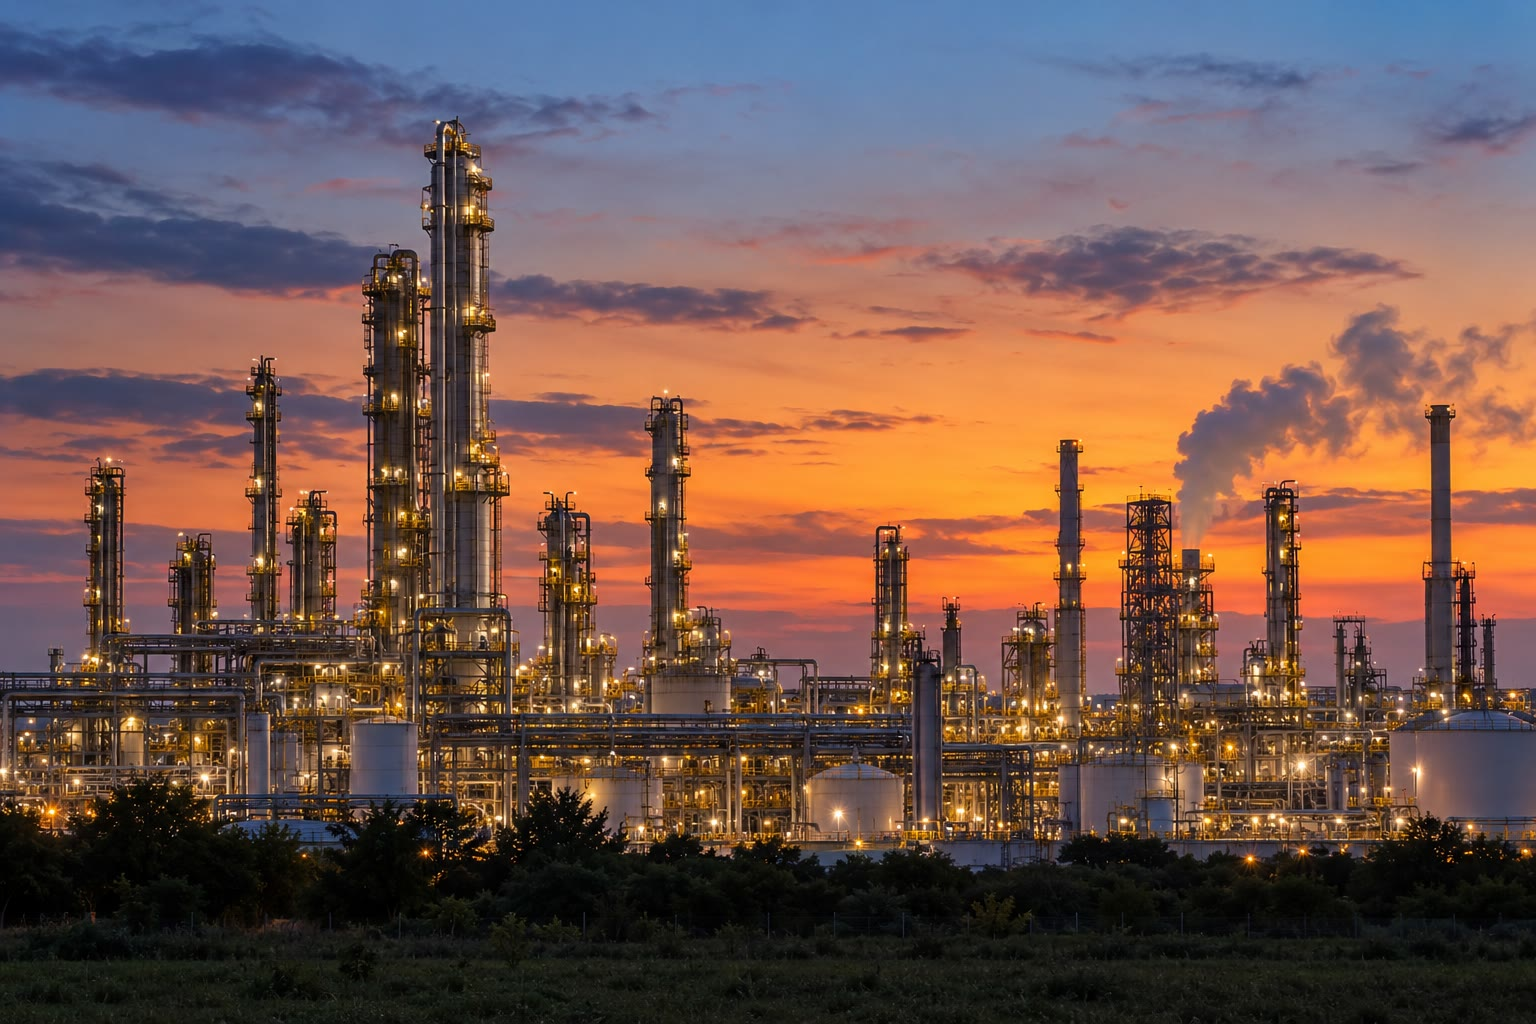
\includegraphics[width=0.6\linewidth]{images/book4/ai/b3-21-chemical-plant.jpg}

{\small A large chemical plant at dusk. In a \omterm{def:b3:homogeneous-catalysis:carbonylation}{carbonylation} unit, the catalyst
is a metal complex dissolved in the reaction liquid; most of the plant
separates and recycles.}
\end{omfigure}

\section{Hydrogenation}

\begin{method}[Reading a catalytic cycle]\label{met:b3:homogeneous-catalysis:read-cycle}
\begin{enumerate}
  \item At each species, count the valence electrons and give the oxidation
        state and $d^n$ of the metal.
  \item Name each step (ligand loss or addition, oxidative addition,
        insertion, elimination) and check that the counts change as it requires
        (oxidative addition: $+2$ in oxidation state and in electron count).
  \item Identify the resting state (the species that accumulates) and the
        rate-determining step; the rate law follows from the pre-equilibria
        between them.
\end{enumerate}
\end{method}

\begin{omfigure}
\begin{tikzpicture}[font=\small, >=Stealth]
  \node (a) at (90:2.3) {\ce{RhCl(PPh3)2} \ (14, Rh$^{\mathrm I}$)};
  \node (b) at (0:3.0) {\ce{RhClH2(PPh3)2} \ (16, Rh$^{\mathrm{III}}$)};
  \node (c) at (-90:2.3) {\ce{RhClH2(RCH=CH2)(PPh3)2} \ (18)};
  \node (d) at (180:3.1) {\ce{RhClH(CH2CH2R)(PPh3)2} \ (16)};
  \draw[->, thick] (a) to[bend left=22] node[midway, above right, font=\scriptsize] {$+\,\ce{H2}$, oxidative addition} (b);
  \draw[->, thick] (b) to[bend left=22] node[midway, below right, font=\scriptsize] {$+$ alkene} (c);
  \draw[->, thick] (c) to[bend left=22] node[midway, below left, font=\scriptsize] {migratory insertion} (d);
  \draw[->, thick] (d) to[bend left=22] node[midway, above left, font=\scriptsize, align=right] {reductive\\ elimination: $-$ alkane} (a);
  \node[anchor=south] (p) at (90:3.4) {\ce{RhCl(PPh3)3} \ (16, precatalyst)};
  \draw[<->, black!50] (p) -- (a) node[midway, right, font=\scriptsize] {$\mp\,\ce{PPh3}$};
\end{tikzpicture}

{\small A simplified cycle of alkene hydrogenation by Wilkinson's catalyst
(valence electron counts in brackets). Loss of a phosphine opens a site; the
cycle adds hydrogen, binds the alkene, inserts it into an Rh--H bond and
eliminates the alkane.}
\end{omfigure}

\begin{proposition}[Wilkinson kinetics]\label{prop:b3:homogeneous-catalysis:wilkinson-rate}
If $\ce{RhClL3} \rightleftharpoons \ce{RhClL2} + \mathrm L$ ($K_1$) and $\ce{RhClL2} + \ce{H2} \rightleftharpoons \ce{RhClH2L2}$ ($K_2$) are fast
equilibria and the reaction of the dihydride with the alkene (rate constant $k$)
is rate-determining,
\[
  v = \frac{kK_1K_2[\mathrm{Rh}]_{\mathrm{tot}}[\ce{H2}][\text{alkene}]}{[\mathrm L] + K_1 + K_1K_2[\ce{H2}]},
\]
which saturates in hydrogen and is inhibited by added phosphine L.
\end{proposition}

\begin{proof}
$[\ce{RhClL2}] = K_1[\ce{RhClL3}]/[\mathrm L]$ and $[\ce{RhClH2L2}] = K_2[\ce{H2}][\ce{RhClL2}]$. Writing $[\mathrm{Rh}]_{\mathrm{tot}}$ as the
sum of the three species and solving for the dihydride gives $[\ce{RhClH2L2}] =
K_1K_2[\ce{H2}][\mathrm{Rh}]_{\mathrm{tot}}/([\mathrm L] + K_1 + K_1K_2[\ce{H2}])$; the rate is $k$ times this and the alkene
concentration.
\end{proof}

Wilkinson's catalyst hydrogenates unhindered alkenes much faster than
substituted ones and leaves carbonyl groups untouched: the selectivity of a
crowded metal centre. Chiral diphosphines turn the same chemistry into
asymmetric hydrogenation (\cref{ch:b3:asymmetric-synthesis}).

\section{Carbonylation processes}

\begin{definition}[Hydroformylation]\label{def:b3:homogeneous-catalysis:hydroformylation}
\emph{Hydroformylation}\index{hydroformylation} is the addition of a hydrogen atom
and a formyl group (CHO) across a C=C double bond, from $\ce{H2}$ and CO, turning an
alkene into an aldehyde with one more carbon. The \emph{linear-to-branched
ratio}\index{linear-to-branched ratio} is the ratio of the straight-chain
aldehyde to the branched one.
\end{definition}

The first processes used $\ce{HCo(CO)4}$ at about 150 to \qty{180}{\celsius} and very high
pressures. Rhodium with triphenylphosphine works at around \qty{100}{\celsius} and
much lower pressures, and gives a higher \omterm{def:b3:homogeneous-catalysis:hydroformylation}{linear-to-branched ratio}: the bulky
phosphines favour the insertion that puts the metal on the terminal carbon.
Propene gives butanal, hydrogenated to butanol or converted to plasticiser
alcohols.

\begin{definition}[Carbonylation]\label{def:b3:homogeneous-catalysis:carbonylation}
\emph{Carbonylation}\index{carbonylation} is the introduction of a carbonyl group
into a molecule by reaction with carbon monoxide, catalysed by a metal complex
through the migratory insertion of CO.
\end{definition}

The \omterm{def:b3:homogeneous-catalysis:carbonylation}{carbonylation} of methanol to acetic acid, $\ce{CH3OH + CO -> CH3COOH}$, runs on
rhodium (the Monsanto process) or iridium (the Cativa process) with methyl iodide
as co-catalyst: hydrogen iodide turns methanol into methyl iodide, the metal
inserts CO into the methyl group, and the acetyl iodide formed is hydrolysed,
releasing HI again.

\begin{omfigure}
\begin{tikzpicture}[font=\small, >=Stealth]
  \node (a) at (90:2.1) {$\ce{[M(CO)2I2]-}$ (16)};
  \node (b) at (0:2.9) {$\ce{[CH3M(CO)2I3]-}$ (18)};
  \node (c) at (-90:2.1) {$\ce{[CH3COM(CO)I3]-}$ (16)};
  \node (d) at (180:2.9) {$\ce{[CH3COM(CO)2I3]-}$ (18)};
  \draw[->, thick] (a) to[bend left=22] node[midway, above right, font=\scriptsize, align=left] {$+\,\ce{CH3I}$\\ oxidative addition} (b);
  \draw[->, thick] (b) to[bend left=22] node[midway, below right, font=\scriptsize] {migratory insertion} (c);
  \draw[->, thick] (c) to[bend left=22] node[midway, below left, font=\scriptsize] {$+$ CO} (d);
  \draw[->, thick] (d) to[bend left=22] node[midway, above left, font=\scriptsize, align=right] {reductive elimination\\ $-\,\ce{CH3COI}$} (a);
  \node[anchor=north, align=center, font=\scriptsize] at (0,-2.55) {$\ce{CH3COI + H2O -> CH3COOH + HI}$, \quad $\ce{CH3OH + HI -> CH3I + H2O}$};
\end{tikzpicture}

{\small The \omterm{def:b3:homogeneous-catalysis:carbonylation}{carbonylation} cycle of methanol for $\mathrm M = \mathrm{Rh}$ (Monsanto); valence
electron counts in brackets, metal oxidation state I at the top, III elsewhere.
With rhodium the oxidative addition of methyl iodide is rate-determining. With
iridium (Cativa) it is much faster, the migratory insertion is slow, and
\omterm{def:b3:surfaces-catalysis:catalyst-design}{promoters} that remove one iodide from $\ce{[CH3Ir(CO)2I3]-}$ speed up the insertion.}
\end{omfigure}

\begin{proposition}[Rate law of the rhodium process]\label{prop:b3:homogeneous-catalysis:monsanto-rate}
If the oxidative addition of methyl iodide to $\ce{[Rh(CO)2I2]-}$ is rate-determining and
this complex is the resting state, $v = k[\mathrm{Rh}]_{\mathrm{tot}}[\ce{CH3I}]$: zero order in CO and in
methanol.
\end{proposition}

\begin{proof}
The rate is that of the slow step, $k[\ce{[Rh(CO)2I2]-}][\ce{CH3I}]$, and almost all the rhodium
is in the resting state. CO enters only after the slow step, and methanol only
regenerates methyl iodide, whose steady concentration is set by the iodide
charged to the reactor rather than by the methanol.
\end{proof}

Iridium won over rhodium in new plants for practical reasons: its complexes stay
in solution at lower water concentrations, which saves energy in drying the
product, and they give fewer by-products. The main side reaction of both is the
water--gas shift, $\ce{CO + H2O -> CO2 + H2}$, catalysed by the same metal, which wastes
carbon monoxide.

\section{Olefin metathesis}

\begin{definition}[Olefin metathesis]\label{def:b3:homogeneous-catalysis:metathesis}
\emph{Olefin metathesis}\index{olefin metathesis} is the exchange of the
alkylidene halves of two alkenes, $\mathrm{RCH{=}CHR + R'CH{=}CHR' \rightleftharpoons 2\,RCH{=}CHR'}$, catalysed by
metal \omterm{def:b3:organometallic-bonding:carbene}{carbene complexes} through a \emph{metallacyclobutane}\index{metallacyclobutane},
a four-membered ring of the metal and three carbons. Its synthetic forms are
\emph{ring-closing metathesis}\index{ring-closing metathesis} (RCM), which joins
two alkene ends of one molecule into a ring with loss of ethene,
\emph{ring-opening metathesis polymerisation}\index{ring-opening metathesis polymerisation}
(ROMP) of strained cyclic alkenes, and \emph{cross
metathesis}\index{cross metathesis} between two different alkenes.
\end{definition}

\begin{definition}[Chauvin mechanism]\label{def:b3:homogeneous-catalysis:chauvin}
The \emph{Chauvin mechanism}\index{Chauvin mechanism} of metathesis is the
$[2+2]$ cycloaddition of an alkene to a metal \omterm{def:b3:organometallic-bonding:carbene}{carbene}, $\mathrm{[M]{=}CHR}$, giving a
\omterm{def:b3:homogeneous-catalysis:metathesis}{metallacyclobutane}, followed by its cycloreversion in the other direction,
which releases a new alkene and a new \omterm{def:b3:organometallic-bonding:carbene}{carbene}.
\end{definition}

\begin{omfigure}
\setchemfig{atom sep=2.1em}
\schemestart
\chemfig{M=[:0]CHR}
\+
\chemfig{R'HC=[:0]CHR'}
\arrow{<=>}
\chemfig{M?-[:0]CHR-[:-90]CHR'-[:180]CHR'?}
\arrow{<=>}
\chemfig{M=[:0]CHR'}
\+
\chemfig{RHC=[:0]CHR'}
\schemestop
\par\vspace{10pt}

{\small The \omterm{def:b3:homogeneous-catalysis:chauvin}{Chauvin mechanism}: a metal \omterm{def:b3:organometallic-bonding:carbene}{carbene} and an alkene combine into a
\omterm{def:b3:homogeneous-catalysis:metathesis}{metallacyclobutane}, which opens the other way to give a new \omterm{def:b3:organometallic-bonding:carbene}{carbene} and a new
alkene. Each step is reversible: metathesis reaches an equilibrium unless a
product leaves.}
\end{omfigure}

\begin{proposition}[Driving ring-closing metathesis]\label{prop:b3:homogeneous-catalysis:metathesis-equilibrium}
For a ring closure $\text{diene} \rightleftharpoons \text{cycloalkene} + \ce{C2H4}$, removing ethene from the
solution drives the reaction to completion; the reaction is favoured by the
entropy of releasing a gas molecule.
\end{proposition}

\begin{proof}
At equilibrium $K = [\text{ring}][\ce{C2H4}]/[\text{diene}]$: if $[\ce{C2H4}]$ is kept low by purging or
evacuating, $[\text{ring}]/[\text{diene}] = K/[\ce{C2H4}]$ grows without limit. The number of molecules
increases by one in the reaction while the bonds made and broken (a C=C each) are
alike: $\Delta_rH^\circ \approx 0$ for an unstrained ring and $\Delta_rS^\circ > 0$, so $K$ is favourable.
\end{proof}

ROMP of strained rings, such as norbornene, runs the other way for the opposite
reason: the release of ring strain pays for the loss of translational entropy.
Robert Grubbs's ruthenium \omterm{def:b3:organometallic-bonding:carbene}{carbenes} tolerate water, air and most functional
groups; Richard Schrock's molybdenum and tungsten alkylidenes are more active
and can be made enantioselective.

\section{Palladium cross-coupling}

\begin{definition}[Cross-coupling reactions]\label{def:b3:homogeneous-catalysis:cross-coupling}
A \emph{cross-coupling reaction}\index{cross-coupling reaction} joins two
different carbon fragments, an organic halide and an organometallic reagent or an
alkene, on a metal catalyst, usually palladium. In the \emph{Heck
reaction}\index{Heck reaction} an aryl or vinyl halide couples with an alkene,
giving a substituted alkene; in the \emph{Suzuki--Miyaura
coupling}\index{Suzuki--Miyaura coupling} it couples with an organoboron
compound in the presence of a base.
\end{definition}

\begin{omfigure}
\begin{tikzpicture}[font=\small, >=Stealth]
  \node (a) at (90:2.0) {$\mathrm{Pd^0L_2}$};
  \node (b) at (0:2.6) {$\mathrm{ArPd^{II}XL_2}$};
  \node (c) at (-90:2.0) {$\mathrm{ArPd^{II}Ar'L_2}$};
  \draw[->, thick] (a) to[bend left=25] node[midway, above right, font=\scriptsize, align=left] {$+\,$ArX\\ oxidative addition} (b);
  \draw[->, thick] (b) to[bend left=25] node[midway, below right, font=\scriptsize, align=left] {$+\,\mathrm{Ar'B(OH)_2}$, base\\ transmetalation} (c);
  \draw[->, thick] (c) to[bend left=35] node[midway, left, font=\scriptsize, align=right] {reductive elimination\\ $-\,$Ar--Ar$'$} (a);
\end{tikzpicture}

{\small The Suzuki--Miyaura cycle: palladium(0) inserts into the C--X bond of the
aryl halide, receives the second aryl group from the boronic acid activated by
the base, and releases the biaryl by reductive elimination.}
\end{omfigure}

\begin{method}[Choosing a cross-coupling]\label{met:b3:homogeneous-catalysis:choose-coupling}
\begin{enumerate}
  \item Disconnect the target at the C--C bond to be made; one partner becomes the
        halide (iodide $>$ bromide $>$ triflate $>$ chloride in reactivity), the other the
        boronic acid (Suzuki--Miyaura), the alkene (Heck), the organozinc
        (Negishi) or the terminal alkyne with copper(I) (Sonogashira).
  \item Prefer the partner pair whose reagents are stable, available and least
        toxic: boronic acids for biaryls.
  \item Choose the ligand for the hardest step: electron-rich, bulky phosphines
        or \omterm{def:b3:organometallic-bonding:carbene}{N-heterocyclic carbenes} speed the oxidative addition of chlorides.
  \item Plan the removal of palladium from the product to the low levels
        allowed in drugs (scavenger resins, crystallisation).
\end{enumerate}
\end{method}

\section{Polymerisation catalysis}

\begin{definition}[Ziegler--Natta catalysis]\label{def:b3:homogeneous-catalysis:ziegler-natta}
A \emph{Ziegler--Natta catalyst}\index{Ziegler--Natta catalyst} polymerises
alkenes at low pressure; it is made from a transition-metal halide, typically of
titanium, and an alkylaluminium compound. The \emph{Cossee--Arlman
mechanism}\index{Cossee--Arlman mechanism} of chain growth is the coordination
of the alkene at a vacant site cis to the growing alkyl chain on the metal,
followed by its migratory insertion into the metal--carbon bond, which leaves a
vacant site again. A \emph{single-site catalyst}\index{single-site catalyst} has
all its active centres identical, as in a molecular \omterm{def:b3:organometallic-bonding:metallocene}{metallocene} catalyst.
\end{definition}

\begin{omfigure}
\begin{tikzpicture}[font=\small, >=Stealth]
  \begin{scope}[every node/.style={inner sep=1pt}]
  % panel 1: chain and vacant site
  \node (m1) at (0,0) {M};
  \node (p1) at (-0.7,0.55) {P};
  \node (v1) at (0.7,0.55) {$\square$};
  \draw (m1) -- (p1);
  % panel 2: alkene bound side-on at the vacant site
  \node (m2) at (3.6,0) {M};
  \node (p2) at (2.9,0.55) {P};
  \node (c2a) at (4.75,1.25) {\ce{CH2}};
  \node (c2b) at (4.75,0.25) {\ce{CH2}};
  \draw (m2) -- (p2);
  \draw[double, double distance=1.6pt] (c2a) -- (c2b);
  \draw[dashed] (m2) -- (4.55,0.75);
  % panel 3: chain longer by two carbons, vacant site moved
  \node (m3) at (7.7,0) {M};
  \node (v3) at (7.0,0.55) {$\square$};
  \node (c3a) at (8.45,0.55) {\ce{CH2}};
  \node (c3b) at (8.45,1.45) {\ce{CH2}};
  \node (p3) at (7.75,1.95) {P};
  \draw (m3) -- (c3a) -- (c3b) -- (p3);
  \end{scope}
  \draw[->, thick] (1.25,0.35) -- (2.55,0.35) node[midway, above, font=\scriptsize] {$+\,\ce{C2H4}$};
  \draw[->, thick] (5.35,0.35) -- (6.3,0.35) node[midway, above, font=\scriptsize] {insertion};
\end{tikzpicture}
\par\medskip

{\small The \omterm{def:b3:homogeneous-catalysis:ziegler-natta}{Cossee--Arlman mechanism} (P: the growing polymer chain; $\square$: a
vacant site). The alkene binds next to the chain and inserts into the M--C
bond through a four-membered transition state; the chain, longer by two
carbons, now occupies the site where the alkene was, and the vacant site has
moved.}
\end{omfigure}

\begin{proposition}[Tacticity from catalyst symmetry]\label{prop:b3:homogeneous-catalysis:tacticity-symmetry}
For a \omterm{def:b3:organometallic-bonding:metallocene}{metallocene} catalyst on which the chain migrates between two coordination
sites at each insertion, a $C_2$-symmetric catalyst gives isotactic
polypropylene and a $C_s$-symmetric catalyst syndiotactic polypropylene.
\end{proposition}

\begin{proof}[Argued]
The face of the propene that inserts is chosen by the chiral environment of the
site. In a $C_2$-symmetric catalyst the two sites are exchanged by the $C_2$ axis,
which preserves handedness (\cref{ch:b3:point-groups}): both sites select the
same face, and successive methyl groups have the same configuration (isotactic).
In a $C_s$-symmetric catalyst the two sites are mirror images: they select opposite
faces, and the configurations alternate (syndiotactic). A catalyst whose sites
are achiral, such as unbridged $\ce{Cp2ZrCl2}$ with methylaluminoxane, gives atactic
polymer.
\end{proof}

\begin{proposition}[Schulz--Flory distribution]\label{prop:b3:homogeneous-catalysis:schulz-flory}
If each growing chain on a \omterm{def:b3:homogeneous-catalysis:ziegler-natta}{single-site catalyst} adds a monomer with constant
probability $p$ and is otherwise transferred (terminated), the number fraction of
chains of $n$ units is $x_n = (1 - p)p^{n-1}$, and the dispersity $M_w/M_n = 1 + p$ tends to 2 for long chains.
\end{proposition}

\begin{proof}
A chain of exactly $n$ units has grown $n - 1$ times and stopped once:
probability $p^{n-1}(1 - p)$. Then $\sum nx_n = 1/(1 - p)$ (number average), and the mass
fractions $w_n = nx_n(1 - p)$ give the mass average $\sum nw_n = (1 + p)/(1 - p)$. Their
ratio is $1 + p$.
\end{proof}

\begin{omfigure}
\begin{tikzpicture}
\begin{axis}[width=0.7\linewidth, height=5.2cm, xmin=0, xmax=200, ymin=0, ymax=1.05,
  axis lines=left, xlabel={$M$ / \unit{kg.mol^{-1}}}, ylabel={fraction per unit (scaled)},
  tick label style={font=\small}, label style={font=\small},
  legend style={font=\scriptsize, draw=none, at={(0.98,0.98)}, anchor=north east}, legend cell align=left]
\addplot[omDef, line width=1pt] table[x=M_kg, y=x] {figdata/out/bachelor-3-schulz-flory.dat};
\addplot[omThm, line width=1pt] table[x=M_kg, y expr=\thisrow{w}/0.368] {figdata/out/bachelor-3-schulz-flory.dat};
\draw[black!40, dashed] (axis cs:28.05,0) -- (axis cs:28.05,1);
\node[font=\scriptsize, anchor=west] at (axis cs:30,0.5) {$M_n$};
\legend{number fraction, mass fraction (scaled to its maximum)}
\end{axis}
\end{tikzpicture}

{\small The most probable molar-mass distribution of a polyethylene made on a
\omterm{def:b3:homogeneous-catalysis:ziegler-natta}{single-site catalyst} (model: mean degree of polymerisation 1000): the number
fraction falls exponentially, the mass fraction peaks at $M_n \approx \qty{28}{kg/mol}$; $M_w = 2M_n$. Classical
\omterm{def:b3:homogeneous-catalysis:ziegler-natta}{Ziegler--Natta catalysts}, with several kinds of sites, give broader
distributions.}
\end{omfigure}

\begin{inthelab}[A Suzuki coupling and its palladium]
The aryl bromide, the boronic acid (1.2 equivalents), potassium carbonate and a
few tenths of a per cent of a palladium phosphine complex are stirred in a
degassed mixture of toluene, ethanol and water under nitrogen at reflux. After
work-up the crude biaryl is stirred with a thiol-functionalised silica that
binds palladium, filtered and crystallised; the palladium left is measured by
plasma mass spectrometry.
\end{inthelab}

\begin{safety}{\ghs[0.62cm]{GHS02}\ghs[0.62cm]{GHS04}\ghs[0.62cm]{GHS06}\ghs[0.62cm]{GHS08}}
% ledger: ghs4:MeI, ghs:CO
Methyl iodide: toxic by inhalation and ingestion, harmful in contact with skin, suspected
carcinogen, volatile; handled in a fume hood. Carbon monoxide: extremely
flammable, toxic by inhalation, may damage the unborn child, odourless; used
with fixed detectors and alarms.
\end{safety}

\begin{history}[Ziegler, Natta, and metathesis]
Karl Ziegler found in 1953 that titanium chloride and alkylaluminium compounds
polymerise ethene at atmospheric pressure, and Giulio Natta in 1954 that such
catalysts make stereoregular polypropylene; they shared the 1963 Nobel Prize in
Chemistry. Yves Chauvin proposed the \omterm{def:b3:homogeneous-catalysis:metathesis}{metallacyclobutane} mechanism of
metathesis in 1971; with Robert Grubbs and Richard Schrock, who made well-defined
metathesis catalysts, he received the 2005 Nobel Prize in Chemistry.
\end{history}

\section{Exercises}

\begin{exercise}[$\star$]\label{exo:b3:homogeneous-catalysis:1}
Give the valence electron count and the oxidation state of rhodium at each step
of the Wilkinson cycle of the figure.
\end{exercise}

\begin{exercise}[$\star$]\label{exo:b3:homogeneous-catalysis:2}
Name the two aldehydes formed by \omterm{def:b3:homogeneous-catalysis:hydroformylation}{hydroformylation} of propene. Which is the linear
one?
\end{exercise}

\begin{exercise}[$\star$]\label{exo:b3:homogeneous-catalysis:3}
Diethyl diallylmalonate, $\ce{(CH2=CHCH2)2C(CO2Et)2}$, undergoes \omterm{def:b3:homogeneous-catalysis:metathesis}{ring-closing metathesis}.
Give the product and the size of its ring.
\end{exercise}

\begin{exercise}[$\star$]\label{exo:b3:homogeneous-catalysis:4}
Give the product of the \omterm{def:b3:homogeneous-catalysis:cross-coupling}{Heck reaction} of iodobenzene with methyl acrylate, and its
configuration.
\end{exercise}

\begin{exercise}[$\star\star$]\label{exo:b3:homogeneous-catalysis:5}
Starting from the cycle of the rhodium process, derive its rate law, and explain
why the methanol conversion does not change the rate until it is nearly complete.
\end{exercise}

\begin{exercise}[$\star\star$]\label{exo:b3:homogeneous-catalysis:6}
Propose two Suzuki--Miyaura disconnections of 4-methylbiphenyl and choose one.
\end{exercise}

\begin{exercise}[$\star\star$]\label{exo:b3:homogeneous-catalysis:7}
Predict the tacticity of polypropylene made with a $C_2$-symmetric bridged
bis(indenyl)zirconium catalyst, a $C_s$-symmetric one, and unbridged $\ce{Cp2ZrCl2}$.
\end{exercise}

\begin{exercise}[$\star\star$]\label{exo:b3:homogeneous-catalysis:8}
With \qty{0.10}{mol\%} of catalyst, a hydrogenation reaches 98\,\% conversion in \qty{2.0}{h}.
Compute the turnover number and the mean turnover frequency.
\end{exercise}

\begin{exercise}[$\star\star$]\label{exo:b3:homogeneous-catalysis:9}
Draw the repeating unit of the polymer made by ring-opening metathesis of
norbornene, and explain why the reaction goes to completion.
\end{exercise}

\begin{exercise}[$\star\star\star$]\label{exo:b3:homogeneous-catalysis:10}
A \omterm{def:b3:homogeneous-catalysis:ziegler-natta}{single-site catalyst} gives chains with $p = 0.9995$. Compute the number-average
degree of polymerisation and the dispersity. Why is a Ziegler--Natta polymer
broader?
\end{exercise}

\begin{exercise}[$\star\star\star$]\label{exo:b3:homogeneous-catalysis:11}
Show from the Wilkinson rate law that the rate is first order in $\ce{H2}$ at low pressure
and independent of it at high pressure, and that adding phosphine slows the
reaction.
\end{exercise}

\begin{exercise}[$\star\star\star$]\label{exo:b3:homogeneous-catalysis:12}
Explain why bulky phosphines raise the \omterm{def:b3:homogeneous-catalysis:hydroformylation}{linear-to-branched ratio} in rhodium
\omterm{def:b3:homogeneous-catalysis:hydroformylation}{hydroformylation}, and why a high ratio matters for the plasticiser alcohols made
from the aldehydes.
\end{exercise}

\section{Problem: From Methanol to Vinegar}

\begin{problem}[{Weekend problem --- from methanol to vinegar on an iridium cycle:
the counts and steps of the cycle, its rate-determining step and promoters, a
plant's turnover frequency, and the carbon monoxide lost to the water--gas
shift}]
\label{pb:b3:homogeneous-catalysis:1}
% ledger: aw:Ir, aw:C, aw:H, aw:O
An acetic acid plant (data of the problem) produces $\qty{5.0e5}{t}$ of acetic acid a year
in \qty{8000}{h} of operation, with \qty{200}{m^3} of reaction liquid containing \qty{5.0}{mmol/L} of
iridium. Its selectivity on carbon monoxide is 94\,\%: the rest is converted by the
water--gas shift.

\medskip\noindent\textbf{Part I --- The cycle.}
\begin{enumerate}
  \item Count the electrons of $\ce{[Ir(CO)2I2]-}$ and give its oxidation state.
  \item Oxidative addition of $\ce{CH3I}$: product, count, oxidation state?
  \item Loss of iodide and addition of CO: what neutral complex forms?
  \item Migratory insertion: product and count?
  \item Addition of iodide, then reductive elimination of acetyl iodide: what is
        regenerated?
  \item Write the two organic steps that close the cycle with water and methanol.
  \item Write the overall reaction.
\end{enumerate}

\medskip\noindent\textbf{Part II --- Kinetics.}
\begin{enumerate}[resume]
  \item Which step is rate-determining with iridium, and how does that differ from
        rhodium?
  \item How do \omterm{def:b3:surfaces-catalysis:catalyst-design}{promoters} that capture iodide accelerate the cycle?
  \item What dependence on the iodide concentration does this predict?
  \item Why is the rate independent of the methanol concentration?
\end{enumerate}

\medskip\noindent\textbf{Part III --- The plant.}
\begin{enumerate}[resume]
  \item Compute the amount of acetic acid made per year.
  \item Compute the amount per hour.
  \item Compute the amount of iridium in the reactor, and its mass.
  \item Compute the turnover frequency.
  \item Compute the turnover number per year.
  \item Compute the space--time yield in kilograms per cubic metre per hour.
\end{enumerate}

\medskip\noindent\textbf{Part IV --- The water--gas shift.}
\begin{enumerate}[resume]
  \item Write the water--gas shift reaction.
  \item Compute the CO consumed per mole of acetic acid.
  \item Compute the \ce{CO2} formed per mole of acetic acid.
  \item Compute the mass of \ce{CO2} emitted per tonne of acetic acid.
  \item Why does running at lower water concentration help, and what limits it?
  \item What other product does the shift make, and why is it a problem in the
        reactor?
  \item State the result: the turnover frequency of the iridium catalyst.
\end{enumerate}
\end{problem}
